\subsection{Alignment Training Linearization}
%As was mentioned in \autoref{mrtproblemdef}, there are many choices of
%\linearizationstrategy~$\ls$ when modeling \surfacerealization~with
%a \sequencetosequence~archictecture. One particular \linearizationstrategy,
%which we call the \alignmenttraining~linearization, yields a controllable \sequencetosequence~model which is capable of following an utterance plan indicating
% the \surfacerealization~order of a \meaningrepresentation's \attributevalues.
%
%
Unlike the {\color{red}arbitrary linearization} used in \autoref{somewhere}, \alignmenttraining~linearization~is not soley a function of $\mr$, but is determined by both $\mr$ and a reference utterance $\utttoks$. Given a $\left(\mr, \utttoks\right)$ pair, the \alignmenttraining~linearization finds a linearization
$\ls$ such that the order of the \attributevalues~in $\ls(\mr)$ corresponds
to the order in which they are realized in $\utttoks$. %Formally, this means that 
%for any $\left(i^{(\ls_k)},j^{(\ls_k)}\right), \left(i^{(\ls_{k+1})},j^{(\ls_{k+1})}\right) \in \denotationset_{\mr,\utttoks}$, we have $j^{(\ls_k)} < i^{(\ls_{k+1})}$.


\autoref{fig:atexamples} shows some examples of the 
\alignmenttraining~linearization, including some special cases. When
linearizing list-valued attributes, for instance, we treat them as distinct
\attributevalue~pairs. Occasionally, we encounter repeated \attributevalues~in the training set, and in that case we include extra \attributevalue~pairs
in the correpsonding location in the linearization. We ignore any instances
of  ungrounded information, as in example \autoref{} where (such and such)
has no explicit representation.  

%\subsubsection{Alignment Training Implementation}

%\begin{algorithm}[t]
    \caption{Alignment Training Linearization Algorithm}
    \label{alg:at}
    \DontPrintSemicolon
    \KwData{\utterance~$\utttoks \in \outSpace$, \attributevalue~tagger $\tagger$}  
    Tag the utterance, $\mathbf{t} \gets \tagger(\utttoks)$.  \label{alg:attag} \\
Split $\mrtags$ into the minimal number of subsequences with the same distinct
tag value, i.e. $\mrtags = \left[\left[ \mrtag_1, \ldots mrtag_j \right] \right]$\\
    Segment $\mathbf{t}$ into $k$ spans by splitting $\mathbf{t}$ on tags mapped to no \attributevalue~(i.e. $t_i = \emptyset$): $\boldsymbol{\hat{t}} = \left[\ldots,\left[t_{{i_k}},t_{i_{k}+1},\ldots, t_{j_k}\right],\ldots\right]$ \\
    Segment each of the $k$ sub-segments into maximal length contiguous
    spans sharing the same tag.
\end{algorithm}




%\hyperref[alg:at]{Algorithm \ref{alg:at}} shows the alignment training algorithm for a training example $(\mr,\utttoks)$. 

In \autoref{fig:at} we show the steps of our procedure for obtaining
the alignment training linearization, given a reference utterance $\utttoks$.
%the intermediate outputs of each line in \hyperref[alg:at]{Algorithm \ref{alg:at}}. %In practice, there are two distinct and important issues when implementing the 
%\alignmenttraining~linearization. 
The first step is 
to tag the utterance tokens 
$\utttoks = \left[\utttok_1,\ldots,\utttok_\uttSize\right]$ 
with a corresponding tag sequence 
$\mrtags=\left[\mrtag_1,\ldots, \mrtag_\uttSize\right]$ where each 
tag $\mrtag_i$ is equal to an \attributevalue~$\mrtok_j \in \mr$ or 
the null tag $\nulltag$. We assume that we have access to such a tagger
$\tagger : \outSpace \rightarrow \inSpace$ (see \autoref{sec:align}
for implementation details). After producing the tag sequence $\mrtags^{(1)} = \tagger\left(\utttoks\right)$ 
%(\hyperref[alg:attag]{Lines \ref{alg:attag}} in \hyperref[alg:at]{Algorithm \ref{alg:at}} and \hyperref[fig:at]{\autoref{fig:at}.b}),
(\hyperref[fig:at]{\autoref{fig:at}b}),
we then group contiguous sequences of tags sharing the same tag value, discarding any null tag sequences to obtain the sequence of subsequences 
$\mrtags^{(2)} = \left[\mrtags^{(1)}_{i_1:j_1},\ldots,\mrtags^{(1)}_{i_\mrSize:j_\mrSize}, \right]$ (\hyperref[fig:at]{\autoref{fig:at}c}).
Finally, $\mrtoks$ is constructed by 
by prepending the \dialogueact~$\mrtok_0$ of $\mr$ to the ordered sequence 
of \attributevalue~pairs $\mrtok_1,\ldots,\mrtok_\mrSize$ implied by $\mrtags^{(1)}_{i_1},\ldots,\mrtags^{(1)}_{i_\mrSize}$ (\hyperref[fig:at]{\autoref{fig:at}d}). 



%~\\~\\
%we then segment $\mrtags^{(1)}$ into contiguous sequences of tags containing no null tags, $\nulltag$, to obtain the sequence of subsequences
%$\mrtags^{(2)}$ (\hyperref[fig:at]{\autoref{fig:at}c}). Each subsequence of
%$\mrtags^{(2)}$ is further split into the longest contiguous tag sequences 
%such that all 
%tags of a segment are equal to the same \attributevalue~pair(\hyperref[fig:at]{\autoref{fig:at}d}). 
%Finally, $\mrtoks$ is constructed by 
%by prepending the \dialogueact~$\mrtok_0$ of $\mr$ to the ordered sequence 
%of \attributevalue~pairs $???$ implied by $\mrtoks^{(3)}$ (\hyperref[fig:at]{\autoref{fig:at}e}). 
%
\tikzset{mynode/.style={anchor=center, minimum height=1.5em, 
      text height=1.5ex, text depth=.25ex, align=center}}

      \begin{figure}[p]
    \fbox{\begin{minipage}{\textwidth}
            ~\\
        \center
        \scalebox{0.75}{
    \begin{tikzpicture}
        \def\titlex{-3.0}
        \def\colwidth{1.25}
        \def\utttitleheight{2}
        \def\uttheightA{0.0}
        \def\uttheightB{-1.0}
        \def\tagtitleheight{-3.0}
        \def\tagheightA{-5.0}
        \def\tagheightB{-6.0}
        \def\nullsegtitleheight{-12.0}
        \def\nullsegheightA{-14.0}
        \def\mrsegtitleheight{-12.0}
        \def\mrsegheightA{-14.0}
        \def\attitleheight{-16.0}
        \def\atheightA{-18.0}
        \def\atheightB{-19.0}



        \def\city{{area=city centre}};
        \def\coffee{{eat\_type=coffee shop}};
       % \def\nulltag{{$\emptyset$}};
        \def\name{{name=Aromi}};
        \def\words{For, coffee, in, the, centre, of, the, city, {,}, try, 
                   Aromi, .};
        \def\tags{\coffee, \coffee, \city, \city, \city, \city, \city, \city,
                     \nulltag, \nulltag, \name, \nulltag};

        %%% Input Utterance
        \node[mynode,anchor=west] at (\titlex*\colwidth,\utttitleheight) 
            {\Large (a) Input Utterance};

        \foreach \w [count=\wi from 1] in \words {
            \node[mynode] at (\wi*\colwidth,\uttheightA) 
                {$\utttok_{\wi}\ifthenelse{\wi = 12}{}{,}$};
            \node[mynode] at (\wi*\colwidth,\uttheightB) {\w};
        }
        \node[mynode] at (0*\colwidth,\uttheightA) {$\utttoks = \Bigg[$};
        \node[mynode] at (12*\colwidth+0.5,\uttheightA) {$\Bigg]$};


        %%% Tagged Utterance
        \node[mynode,anchor=west] at (\titlex*\colwidth,\tagtitleheight) 
            {\Large (b) Tagged Utterance};
        \foreach \t [count=\ti from 1] in \tags {
            \node[mynode] at (\ti*\colwidth,\tagheightA) 
                {$\mrtag_{\ti}\ifthenelse{\ti = 12}{}{,}$};
            \node[mynode,rotate=90,anchor=east] at 
                (\ti*\colwidth,\tagheightB) {\t};
        }
        \node[mynode] at (0*\colwidth,\tagheightA) {$\mrtags^{(1)} = \Bigg[$};
        \node[mynode] at (12*\colwidth+0.5,\tagheightA) {$\Bigg]$};


%        %%% Null Segmented Tags
%        \node[mynode,anchor=west] at (\titlex*\colwidth,\nullsegtitleheight) 
%            {\Large (c) Null Segmented Tags};
%        \node[mynode] at (0*\colwidth,\nullsegheightA) 
%            {$\mrtags^{(2)} = \Bigg[$};
%        \node[mynode] at (12*\colwidth+0.5,\nullsegheightA) {$\Bigg]$};        
%        \foreach \tprime in {1,...,8} {
%            \node[mynode] at (\tprime*\colwidth,\nullsegheightA) 
%            {$\mrtag_{\tprime}\ifthenelse{\tprime = 8}{}{,}$};
%        }
%        \foreach \tprime in {11} {
%            \node[mynode] at (\tprime*\colwidth,\nullsegheightA) 
%                {$\mrtag_{\tprime}$};
%        }
%
%        \node[mynode] at (\colwidth-0.50,\nullsegheightA) {$\bigg[$};
%        \node[mynode] at (8*\colwidth+0.50,\nullsegheightA) {$\bigg],$};
%        \node[mynode] at (11*\colwidth-0.50,\nullsegheightA) {$\bigg[$};
%        \node[mynode] at (11*\colwidth+0.50,\nullsegheightA) {$\bigg]$};


        %%% MR Segmented Tags
        \node[mynode,anchor=west] at (\titlex*\colwidth,\mrsegtitleheight) 
            {\Large (c) MR Segmented Tags};
        \node[mynode] at (0*\colwidth,\mrsegheightA) 
            {$\mrtags^{(2)} = \Bigg[$};
        \node[mynode] at (12*\colwidth+0.5,\mrsegheightA) {$\Bigg]$};        
        \foreach \tprime in {1,...,2} {
            \node[mynode] at (\tprime*\colwidth,\mrsegheightA) 
            {$\mrtag_{\tprime}\ifthenelse{\tprime = 2}{}{,}$};
        }
        \foreach \tprime in {3,...,8} {
            \node[mynode] at (\tprime*\colwidth,\mrsegheightA) 
            {$\mrtag_{\tprime}\ifthenelse{\tprime = 8}{}{,}$};
        }
        \foreach \tprime in {11} {
            \node[mynode] at (\tprime*\colwidth,\mrsegheightA) 
                {$\mrtag_{\tprime}$};
        }

        \node[mynode] at (\colwidth-0.50,\mrsegheightA) {$\bigg[$};
        \node[mynode,anchor=center] at (2*\colwidth+0.65,\mrsegheightA) {$\Bigg]_1, \Bigg[$};
    \node[mynode] at (8*\colwidth+0.50,\mrsegheightA) {$\bigg]_2,$};
        \node[mynode] at (11*\colwidth-0.50,\mrsegheightA) {$\bigg[$};
        \node[mynode] at (11*\colwidth+0.50,\mrsegheightA) {$\bigg]_3$};


        %%% Alignment Training Linearization
        \node[mynode,anchor=west] at (\titlex*\colwidth,\attitleheight) 
            {\Large (d) Alignment Training Linearization};
        \node[mynode,anchor=east] at (-1.5*\colwidth-0.5,\atheightA) 
            {$\mrtoks = \Bigg[$};
        \node[mynode] at (-1.5*\colwidth,\atheightA) {$\mrtok_0,$};
        \node[mynode] at (1.5*\colwidth,\atheightA) {$\mrtok_1,$};
        \node[mynode] at (5.5*\colwidth,\atheightA) {$\mrtok_2,$};
        \node[mynode] at (11*\colwidth,\atheightA) {$\mrtok_3$};
        \node[mynode] at (11*\colwidth+0.5,\atheightA) {$\Bigg]$};
%
        \node[mynode] at (-1.5*\colwidth,\atheightB) {inform,};
        \node[mynode] at (1.5*\colwidth,\atheightB) {eat\_type=coffee shop,};
        \node[mynode] at (5.5*\colwidth,\atheightB) {area=city centre,};
        \node[mynode] at (11*\colwidth,\atheightB) {name=Aromi};



    \end{tikzpicture}
    }
    ~\\
    \caption{Example steps of the \alignmenttraining~linearization algorithm
        for producing a linearized \meaningrepresentation~$\mrtoks$.}
        \label{fig:at}
\end{minipage}}
\end{figure}




At test time, the generation model is only
presented with a \meaningrepresentation~$\mr$ and we don't have a reference 
utterance $\utttoks$ with which to apply the alignment training 
linearization. In this case,
we can use an utterance planning model $\planner : \mrspace \rightarrow \inSpace$ to map a \meaningrepresentation~$\mr$ to a
linear sequence $\mrtoks$. Alternatively, we can use the test set reference
to obtain the alignment training linearization; this represents an unrealistically
optimistic case where the model has clairvoyant known of the discourse
ordering preferred by a human.
%
%a human reference utterance. In the latter case, this represents an
%unrealistic case where the model has clairvoyant knowledge of the 
%discourse ordering of the desired utterance but is also representative
%of discourse orderings prefered by humans. 
In either case, we refer to 
a linearization $\mrtoks$ obtained either from $\planner$ or a human reference
as an \utteranceplan~since a generation model trained with
\alignmenttraining~linearizations will attempt to follow it during 
the generation of the utterance.



\subsubsection{Alternative Linearization Strategies}

In our experiments, we compare alignment training to three other 
linearization strategies, which we describe below. 
These linearizations, while sensible methods of mapping a 
\meaningrepresentation~to a linear sequence of tokens, have no 
correspondence between the
\meaningrepresentation~linearization and surface realization order. Because
of this, \sequencetosequence~models trained using these linearization strategies are not controllable. These linearization strategies may have some effect on the faithfulness when
compared to each other and alignemnt training, so evaluation of this modelling choice has
additional benefits beyond benchmarking alignment training.
See \autoref{fig:linstrats} for examples of the
different linearization strategies on the same \meaningrepresentation/utterance
pair.
%Crucially, \alignmenttraining~stands in contrast to these 
%alternative linea
%three strategies
%(\lsshort{Rnd}, \lsshort{If}, and \lsshort{Fp}) which do not have any
%correspondence between the the order of attribute-value pairs in $\lin(\mr)$
%and the order in which they are realized in the corresponding
%utterance $\utttoks$.



\paragraph{Random (\textsc{Rnd})} In the \textsc{Random} linearization (\textsc{Rnd}), we randomly
order the attribute-value pairs for a given \meaningrepresentation. This strategy 
serves as a baseline for determining
if linearization ordering matters at all for faithfulness. \textsc{Rnd} 
is similar to token level noise used in
sequential denoising autoencoders \citep{wang2019denoising} and might even improve faithfulness.
During training, we resample the ordering for each example at every epoch
so as not to over fit to a particular random ordering.
We do not resample the validation set in order to obtain stable results 
from which to pick the best model.


\newtcbox{\mybox}[1][]{colframe=blue, colback=blue!15, 
                       nobeforeafter, tcbox raise base, shrink tight, extrude 
                       by=0.75mm, #1}



\begin{figure}
    \center
    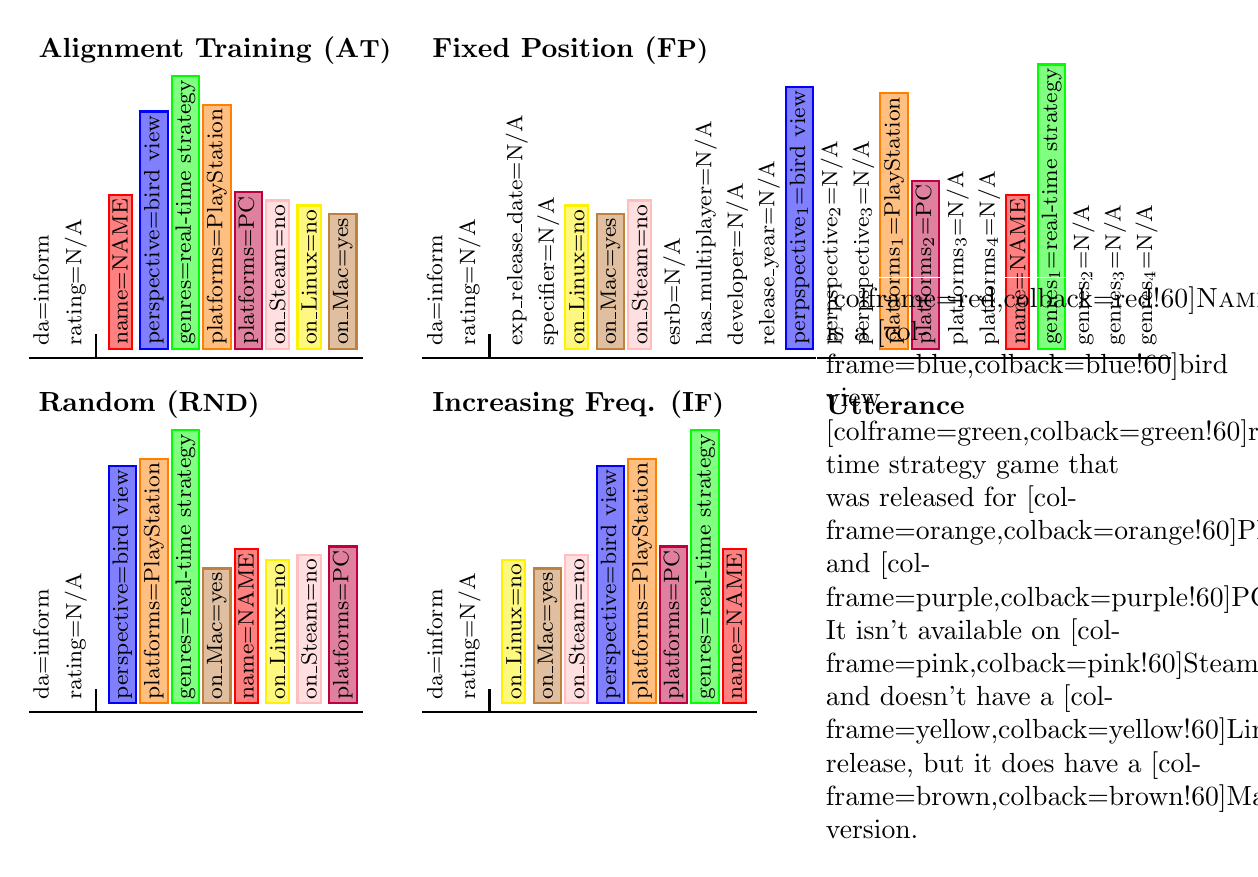
\begin{tikzpicture}[]


    \node[anchor=west] at (5.0,5.8) 
        {\textbf{Fixed Position \textsc{(F\small{P})}}};
    \node[anchor=west] at (0.0,5.8) 
        {\textbf{Alignment Training \textsc{(A\small{T})}}};
    \draw[thick] (0.85,1.9) -- (0.85,2.2);
    \draw[thick] (0,1.9) -- (4.25,1.9);
    \draw[thick] (5 + 0.85,1.9) -- (5 + 0.85,2.2);
    \draw[thick] (5 + 0,1.9) -- (10.25+ 4.25,1.9);
    \draw[thick] (0.85,-2.6) -- (0.85,-2.3);
    \draw[thick] (0,-2.6) -- (4.25,-2.6);
    \draw[thick] (5+0.85,-2.6) -- (5+0.85,-2.3);
    \draw[thick] (5+0,-2.6) -- (5+4.25,-2.6);

    \node[anchor=north west,inner sep=0.5mm,rotate=90] at (0,2) 
        {\footnotesize da=inform};
    \node[anchor=north west,inner sep=0.5mm,rotate=90] at (0.4,2) 
        {\footnotesize rating=N/A};
    \node[anchor=north west,rotate=90,inner sep=0.5mm,draw=red,thick,fill=red!50] 
        at (0.2 + 0.8,2) 
        {\footnotesize name=NAME};
    \node[anchor=north west,rotate=90,inner sep=0.5mm,draw=blue,thick,fill=blue!50] 
        at (0.2 + 1.2,2) {\footnotesize perspective=bird view};
    \node[anchor=north west,rotate=90,inner sep=0.5mm,draw=green,thick,
          fill=green!50] 
        at (0.2 + 1.6,2) {\footnotesize genres=real-time strategy};
    \node[anchor=north west,rotate=90,inner sep=0.5mm,draw=orange,thick,
          fill=orange!50] 
        at (0.2 + 2.0,2) {\footnotesize platforms=PlayStation};
    \node[anchor=north west,rotate=90,inner sep=0.5mm,draw=purple,thick,
          fill=purple!50] 
        at (0.2 + 2.4,2) {\footnotesize platforms=PC};
    \node[anchor=north west,rotate=90,inner sep=0.5mm,draw=pink,thick,
          fill=pink!50] 
        at (0.2 + 2.8,2) {\footnotesize on\_Steam=no};
    \node[anchor=north west,rotate=90,inner sep=0.5mm,draw=yellow,thick,
          fill=yellow!50] 
        at (0.2 + 3.2,2) {\footnotesize on\_Linux=no};
    \node[anchor=north west,rotate=90,inner sep=0.5mm,draw=brown,thick,
          fill=brown!50] 
        at (0.2 + 3.6,2) {\footnotesize on\_Mac=yes};


\node[anchor=north west,inner sep=0.5mm,rotate=90] at (5 + 0,2) 
    {\footnotesize da=inform};
\node[anchor=north west,inner sep=0.5mm,rotate=90] at (5 + 0.4,2) 
    {\footnotesize rating=N/A};
\node[anchor=north west,rotate=90,inner sep=0.5mm] 
    at (5.2 + 0.8,2) 
    {\footnotesize exp\_release\_date=N/A};
\node[anchor=north west,rotate=90,inner sep=0.5mm] 
    at (5.2 + 1.2,2) 
    {\footnotesize specifier=N/A};
\node[anchor=north west,rotate=90,inner sep=0.5mm,draw=yellow,thick,fill=yellow!50] 
    at (5.2 + 1.6,2) 
    {\footnotesize on\_Linux=no};
\node[anchor=north west,rotate=90,inner sep=0.5mm,draw=brown,thick,fill=brown!50] 
    at (5.2 + 2.0,2) 
    {\footnotesize on\_Mac=yes};
\node[anchor=north west,rotate=90,inner sep=0.5mm,draw=pink,thick,fill=pink!50] 
    at (5.2 + 2.4,2) 
    {\footnotesize on\_Steam=no};
\node[anchor=north west,rotate=90,inner sep=0.5mm] 
    at (5.2 + 2.8,2) 
    {\footnotesize esrb=N/A};
\node[anchor=north west,rotate=90,inner sep=0.5mm] 
    at (5.2 + 3.2,2) 
    {\footnotesize has\_multiplayer=N/A};

   % ['inform', 'rating=N/A', 'exp_release_date=N/A', 'specifier=N/A', 'has_linux_release=no', 'has_mac_release=yes', 'available_on_steam=no', 'esrb=N/A', 'has_multiplayer=N/A', 'developer=N/A', 'release_year=N/A', 'player_perspective=bird view', 'player_perspective=N/A', 'player_perspective=N/A', 'platforms=PlayStation', 'platforms=PC', 'platforms=N/A', 'platforms=N/A', 'name=PLACEHOLDER', 'genres=real-time strategy', 'genres=N/A', 'genres=N/A', 'genres=N/A']
\node[anchor=north west,rotate=90,inner sep=0.5mm] 
    at (5.2 + 3.6,2) 
    {\footnotesize developer=N/A};
\node[anchor=north west,rotate=90,inner sep=0.5mm] 
    at (5.2 + 4.0,2) 
    {\footnotesize release\_year=N/A};
\node[anchor=north west,rotate=90,inner sep=0.5mm,draw=blue,thick,fill=blue!50] 
    at (5.2 + 4.4,2) 
    {\footnotesize perpspective\textsubscript{1}=bird view};
\node[anchor=north west,rotate=90,inner sep=0.5mm] 
    at (5.2 + 4.8,2) 
    {\footnotesize perpspective\textsubscript{2}=N/A};
\node[anchor=north west,rotate=90,inner sep=0.5mm] 
    at (5.2 + 5.2,2) 
    {\footnotesize perpspective\textsubscript{3}=N/A};
\node[anchor=north west,rotate=90,inner sep=0.5mm,draw=orange,thick,fill=orange!50] 
    at (5.2 + 5.6,2) 
    {\footnotesize platforms\textsubscript{1}=PlayStation};
\node[anchor=north west,rotate=90,inner sep=0.5mm,draw=purple,thick,fill=purple!50] 
    at (5.2 + 6.0,2) 
    {\footnotesize platforms\textsubscript{2}=PC};
\node[anchor=north west,rotate=90,inner sep=0.5mm] 
    at (5.2 + 6.4,2) 
    {\footnotesize platforms\textsubscript{3}=N/A};
\node[anchor=north west,rotate=90,inner sep=0.5mm] 
    at (5.2 + 6.8,2) 
    {\footnotesize platforms\textsubscript{4}=N/A};
\node[anchor=north west,rotate=90,inner sep=0.5mm,draw=red,thick,fill=red!50] 
    at (5.2 + 7.2,2) 
    {\footnotesize name=NAME};
\node[anchor=north west,rotate=90,inner sep=0.5mm,draw=green,thick,fill=green!50] 
    at (5.2 + 7.6,2) 
    {\footnotesize genres\textsubscript{1}=real-time strategy};
\node[anchor=north west,rotate=90,inner sep=0.5mm] 
    at (5.2 + 8.0,2) 
    {\footnotesize genres\textsubscript{2}=N/A};
\node[anchor=north west,rotate=90,inner sep=0.5mm] 
    at (5.2 + 8.4,2) 
    {\footnotesize genres\textsubscript{3}=N/A};
\node[anchor=north west,rotate=90,inner sep=0.5mm] 
    at (5.2 + 8.8,2) 
    {\footnotesize genres\textsubscript{4}=N/A};


%\node[anchor=north west,rotate=90] at (1.5,2) {genres=platformer};
%\node[anchor=north west,rotate=90] at (2,2) {genres=puzzle};
%\node[anchor=north west,rotate=90] at (2.5,2) {perspective=side vew};
%\node[anchor=north west,rotate=90] at (3,2) {name=NAME};
%\node[anchor=north west,rotate=90] at (3.5,2) {name=NAME};
%\node[anchor=north west,rotate=90] at (4,2) {name=NAME};
%\node[anchor=north west,rotate=90] at (4.5,2) {name=NAME};
%
%
%\node[anchor=north west,rotate=90] at (5.5+0,2) {\small give opinion};
%\node[anchor=north west,rotate=90] at (5.5+0.5,2) {\small rating=good};
%\node[anchor=north west,rotate=90] at (5.5+1,2) {\small genres=adventure};
%\node[anchor=north west,rotate=90] at (5.5+1.5,2) {genres=platformer};
%\node[anchor=north west,rotate=90] at (5.5+2,2) {genres=puzzle};
%\node[anchor=north west,rotate=90] at (5.5+2.5,2) {perspective=side vew};
%\node[anchor=north west,rotate=90] at (5.5+3,2) {name=NAME};
%\node[anchor=north west,rotate=90] at (5.5+3.5,2) {name=NAME};
%\node[anchor=north west,rotate=90] at (5.5+4,2) {name=NAME};
%\node[anchor=north west,rotate=90] at (10+0,2) {give opinion};
%\node[anchor=north west,rotate=90] at (10+0.5,2) {rating=good};
%\node[anchor=north west,rotate=90] at (10+1,2) {genres=adventure};
%\node[anchor=north west,rotate=90] at (10+1.5,2) {genres=platformer};
%\node[anchor=north west,rotate=90] at (10+2,2) {genres=puzzle};
%\node[anchor=north west,rotate=90] at (10+2.5,2) {perspective=side vew};
%\node[anchor=north west,rotate=90] at (10+3,2) {name=NAME};
%\node[anchor=north west,rotate=90] at (10+3.5,2) {name=NAME};
%\node[anchor=north west,rotate=90] at (10+4,2) {name=NAME};
%\node[anchor=north west,rotate=90] at (10+4.5,2) {name=NAME};
%
%



%['give_opinion', 'rating=good', 'genres=adventure', 'genres=platformer', 'genres=puzzle', 'player_perspective=side view', 'name=PLACEHOLDER']


%#
%#

%['inform', 'rating=N/A', 'exp_release_date=N/A', 'specifier=N/A', 'has_linux_release=no', 'has_mac_release=yes', 'available_on_steam=no', 'esrb=N/A', 'has_multiplayer=N/A', 'developer=N/A', 'release_year=N/A', 'player_perspective=bird view', 'player_perspective=N/A', 'player_perspective=N/A', 'platforms=PlayStation', 'platforms=PC', 'platforms=N/A', 'platforms=N/A', 'name=PLACEHOLDER', 'genres=real-time strategy', 'genres=N/A', 'genres=N/A', 'genres=N/A']


%inc_freq_delex
%['inform', 'rating=N/A', 'has_linux_release=no', 'has_mac_release=yes', 'available_on_steam=no', 'player_perspective=bird view', 'platforms=PlayStation', 'platforms=PC', 'name=PLACEHOLDER', 'genres=real-time strategy']

\node[anchor=north west,inner sep=0.5mm,rotate=90] at (0,-2.5) 
    {\footnotesize da=inform};
\node[anchor=north west,inner sep=0.5mm,rotate=90] at (0.4,-2.5) 
    {\footnotesize rating=N/A};
\node[anchor=north west,rotate=90,inner sep=0.5mm,draw=blue,thick,fill=blue!50] 
    at (0.2 + 0.8,-2.5) 
    {\footnotesize perspective=bird view};

\node[anchor=north west,rotate=90,inner sep=0.5mm,draw=orange,thick,fill=orange!50] 
    at (0.2 + 1.2,-2.5) 
    {\footnotesize platforms=PlayStation};
\node[anchor=north west,rotate=90,inner sep=0.5mm,draw=green,thick,fill=green!50] 
    at (0.2 + 1.6,-2.5) 
    {\footnotesize genres=real-time strategy};


\node[anchor=north west,rotate=90,inner sep=0.5mm,draw=brown,thick,fill=brown!50] 
    at (0.2 + 2.0,-2.5) 
    {\footnotesize on\_Mac=yes};
\node[anchor=north west,rotate=90,inner sep=0.5mm,draw=red,thick,fill=red!50] 
    at (0.2 + 2.4,-2.5) 
    {\footnotesize name=NAME};

\node[anchor=north west,rotate=90,inner sep=0.5mm,draw=yellow,thick,fill=yellow!50] 
    at (0.2 + 2.8,-2.5) 
    {\footnotesize on\_Linux=no};
\node[anchor=north west,rotate=90,inner sep=0.5mm,draw=pink,thick,fill=pink!50] 
    at (0.2 + 3.2,-2.5) 
    {\footnotesize on\_Steam=no};
\node[anchor=north west,rotate=90,inner sep=0.5mm,draw=purple,thick,fill=purple!50] 
    at (0.2 + 3.6,-2.5) 
    {\footnotesize platforms=PC};

    \node[anchor=west] at (0,1.3) {\textbf{Random \textsc{(R\small{ND})}}};



\node[anchor=north west,inner sep=0.5mm,rotate=90] at (5 + 0,-2.5) 
    {\footnotesize da=inform};
\node[anchor=north west,inner sep=0.5mm,rotate=90] at (5 + 0.4,-2.5) 
    {\footnotesize rating=N/A};
\node[anchor=north west,rotate=90,inner sep=0.5mm,draw=yellow,thick,fill=yellow!50] 
    at (5.2 + 0.8,-2.5) 
    {\footnotesize on\_Linux=no};
\node[anchor=north west,rotate=90,inner sep=0.5mm,draw=brown,thick,fill=brown!50] 
    at (5.2 + 1.2,-2.5) 
    {\footnotesize on\_Mac=yes};
\node[anchor=north west,rotate=90,inner sep=0.5mm,draw=pink,thick,fill=pink!50] 
    at (5.2 + 1.6,-2.5) 
    {\footnotesize on\_Steam=no};

\node[anchor=north west,rotate=90,inner sep=0.5mm,draw=blue,thick,fill=blue!50]
    at (5.2 + 2.0,-2.5) 
    {\footnotesize perspective=bird view};
\node[anchor=north west,rotate=90,inner sep=0.5mm,draw=orange,thick,fill=orange!50] 
    at (5.2 + 2.4,-2.5) 
    {\footnotesize platforms=PlayStation};
\node[anchor=north west,rotate=90,inner sep=0.5mm,draw=purple,thick,fill=purple!50] 
    at (5.2 + 2.8,-2.5) 
    {\footnotesize platforms=PC};

\node[anchor=north west,rotate=90,inner sep=0.5mm,draw=green,thick,fill=green!50] 
    at (5.2 + 3.2,-2.5) 
    {\footnotesize genres=real-time strategy};
\node[anchor=north west,rotate=90,inner sep=0.5mm,draw=red,thick,fill=red!50] 
    at (5.2 + 3.6,-2.5) 
    {\footnotesize name=NAME};
%has_linux_release=no', 'has_mac_release=yes', 'available_on_steam=no', 'player_perspective=bird view', 'platforms=PlayStation', 'platforms=PC', 'name=PLACEHOLDER', 'genres=real-time strategy'
    \node[anchor=west] at (5.0,1.3) {\textbf{Increasing Freq. \textsc{(I\small{F})}}};


%\node[anchor=north west,inner sep=0.5mm,rotate=90] at (10 + 0,-2.5) 
%    {\footnotesize da=inform};
%\node[anchor=north west,inner sep=0.5mm,rotate=90] at (10 + 0.4,-2.5) 
%    {\footnotesize rating=N/A};
%
%\node[anchor=north west,rotate=90,inner sep=0.5mm,draw=red,thick,fill=red!50] 
%    at (10.2 + 0.8,-2.5) 
%    {\footnotesize name=NAME};
%
%\node[anchor=north west,rotate=90,inner sep=0.5mm,draw=green,thick,fill=green!50] 
%    at (10.2 + 1.2,-2.5) 
%    {\footnotesize genres=real-time strategy};
%
%    \node[anchor=north west,rotate=90,inner sep=0.5mm,draw=purple,thick,fill=purple!50] 
%    at (10.2 + 1.6,-2.5) 
%    {\footnotesize platforms=PC};
%\node[anchor=north west,rotate=90,inner sep=0.5mm,draw=orange,thick,fill=orange!50] 
%    at (10.2 + 2.0,-2.5) 
%    {\footnotesize platforms=PlayStation};
%
%\node[anchor=north west,rotate=90,inner sep=0.5mm,draw=blue,thick,fill=blue!50]
%    at (10.2 + 2.4,-2.5) 
%    {\footnotesize perspective=bird view};
%\node[anchor=north west,rotate=90,inner sep=0.5mm,draw=pink,thick,fill=pink!50] 
%    at (10.2 + 2.8,-2.5) 
%    {\footnotesize on\_Steam=no};
%\node[anchor=north west,rotate=90,inner sep=0.5mm,draw=brown,thick,fill=brown!50] 
%    at (10.2 + 3.2,-2.5) 
%    {\footnotesize on\_Mac=yes};
%\node[anchor=north west,rotate=90,inner sep=0.5mm,draw=yellow,thick,fill=yellow!50] 
%    at (10.2 + 3.6,-2.5) 
%    {\footnotesize on\_Linux=no};
%




%has_linux_release=no', 'has_mac_release=yes', 'available_on_steam=no', 'player_perspective=bird view', 'platforms=PlayStation', 'platforms=PC', 'name=PLACEHOLDER', 'genres=real-time strategy'
%    \node[anchor=west] at (10.0,1.3) {\textbf{Decreasing Freq.}};




    \node[anchor=west] at (10, 1.3) {\textbf{Utterance}};
\node[text width=5.0cm,draw=white,anchor=west] at (10,-0.7) {
    {\mybox[colframe=red,colback=red!60]{\textsc{Name}}} is a 
    \mybox[colframe=blue,colback=blue!60]{bird view} 
    \mybox[colframe=green,colback=green!60]{real-time strategy} 
    game that was released for 
    \mybox[colframe=orange,colback=orange!60]{PlayStation} and 
    \mybox[colframe=purple,colback=purple!60]{PC.} It isn't available on 
    \mybox[colframe=pink,colback=pink!60]{Steam} and doesn't have a 
    \mybox[colframe=yellow,colback=yellow!60]{Linux} release, but it does have
    a \mybox[colframe=brown,colback=brown!60]{Mac} version.
};


\end{tikzpicture}

\caption{Example \meaningrepresentation~linearization strategies for an utterance (lower right) from the 
    ViGGO training set.}
\label{fig:linstrats}
\end{figure}


\paragraph{Increasing Frequency (\textsc{If})} 
In the \textsc{Increasing Frequency} linearization (\textsc{If}), 
we order the attribute-value pairs by increasing frequency of 
occurrence in the training data
i.e. $\acount(\attr_i=\aval_i) \le \acount(\attr_{i+1}=\aval_{i+1})$.
We hypothesize that placing frequently occurring items in a consistent location
may make it easier for the generation model to realize those items correctly, possibly
at the expense of rarer items.

\paragraph{Fixed Position (\textsc{Fp})} We take  consistency one step further 
and create a fixed ordering of all attributes, \textit{n.b.} not attribute-values, ordering them in increasing
frequency of occurrence on the training set (i.e. every instance has the same
order of attributes in the encoder input). In this \textsc{Fixed Position}
linearization (\textsc{Fp}), attributes that are not present 
in an \meaningrepresentation~are explicitly represented with an \textit{N/A} value. 
For list-valued slots, we determine the maximum length list in the training
data and create that many repeated slots in the input sequence.
This linearization is feasible for datasets with a modest number of 
unique attributes (in our case ViGGO has 14 attributes and
the E2E Challenge corpus has eight) but would not easily scale to 10s, 100s, or larger
attribute vocabularies. 





